\documentclass{article}
\usepackage{bm}
\usepackage{amsmath}
\usepackage{graphicx}

\title{Two-Dimensional Dendritic Growth Using Phase-Field Model \\ Report}
\date{2015-Dec-14}
\author{CS 294-73 Group H}

\begin{document}
\pagenumbering{arabic}
\maketitle
    
\section{Stability Constrain}
The stability of the diffusion of the $\phi$ is basing on the $\frac{h^2}{dt}$



\section{Parameter Effect on Dendritic Growth}
The following existing classes will be directly utilized:
\begin{description}
\item[Point, Box, RectMDarray]
\item[VisitWriter, WriteRectMDArray]
\item[CH\_Timer]
\end{description}
A new class \texttt{DendriticGrowth} is defined, along with a modified version of the original \texttt{RK4}. Inside \texttt{DendriticGrowth}, public member data and functions contain $\phi$ and $u$ fields, as well as update and increment functions for both fields. As \texttt{DendriticGrowth} is the only input class for \texttt{RK4}, class setup in \texttt{RK4} is modified accordingly. 

\section{Algorithm and Flow Chart}
\begin{figure}[htb!]
\begin{center}
%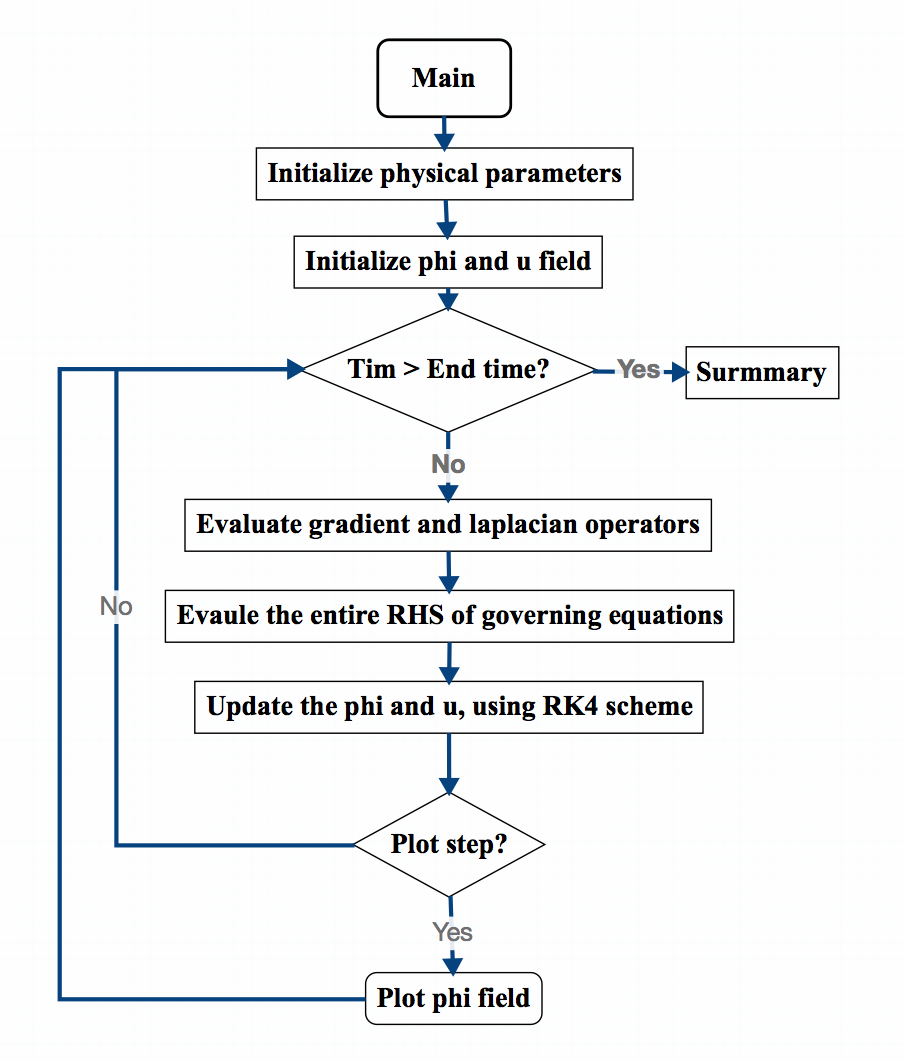
\includegraphics[width=0.8\textwidth]{flowchart_v_1} % Include the image placeholder.png
\caption{Pseudo code diagram for dendritic growth using phase-field model}
\end{center}
\end{figure}
\par \ 
\par 1. Initialize the modeling parameters including timestep dt, end time t, grid dh, domain size L, etc.;
\par 2. Initialize the $\phi$ and $u$ field;
\par 3. Evaluate the gradient and laplacian operators by 2nd order central difference scheme; 
\par 4. Evaluate the orientation angle $\theta$ and $W$;
\par 5. Evaluate RHS of $\phi$ and $u$ euqations, update $\phi$ and $u$ using RK4;
\par 6. Plot intermidiate time step contour of $\phi$ and $u$.
\end{document}